%!TEX root = ../tesis.tex
La propuesta de este trabajo se basa en la extensión del algoritmo de \textit{watershed} en el espacio de color CIELab utilizando la distancia a un punto de referencia. La Figura \ref{img:flujo} muestra el flujo de trabajo propuesto. 
\begin{figure*}[h!]
\centering
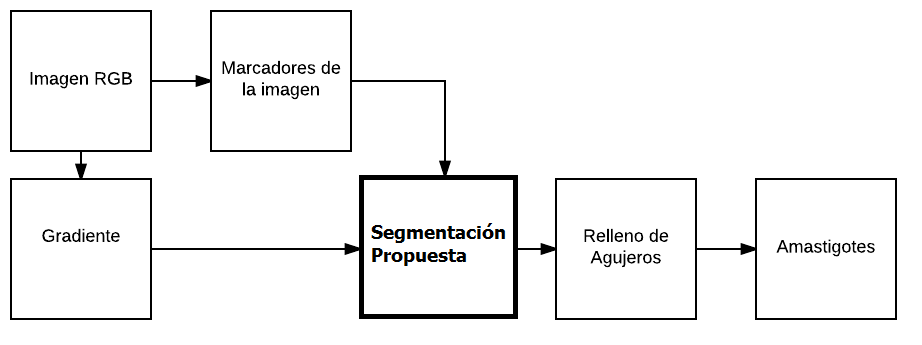
\includegraphics[height=50mm]{./figuras/flujo.png}
\caption{Flujo del trabajo propuesto}
\label{img:flujo}
\end{figure*}
El proceso de la segmentación propuesta está compuesta de varios procesos como se muestran en la Figura \ref{img:segpropuesta}, que se explican posteriormente en el Algoritmo \ref{algoritmo}. 
\begin{figure*}[h!]
\centering
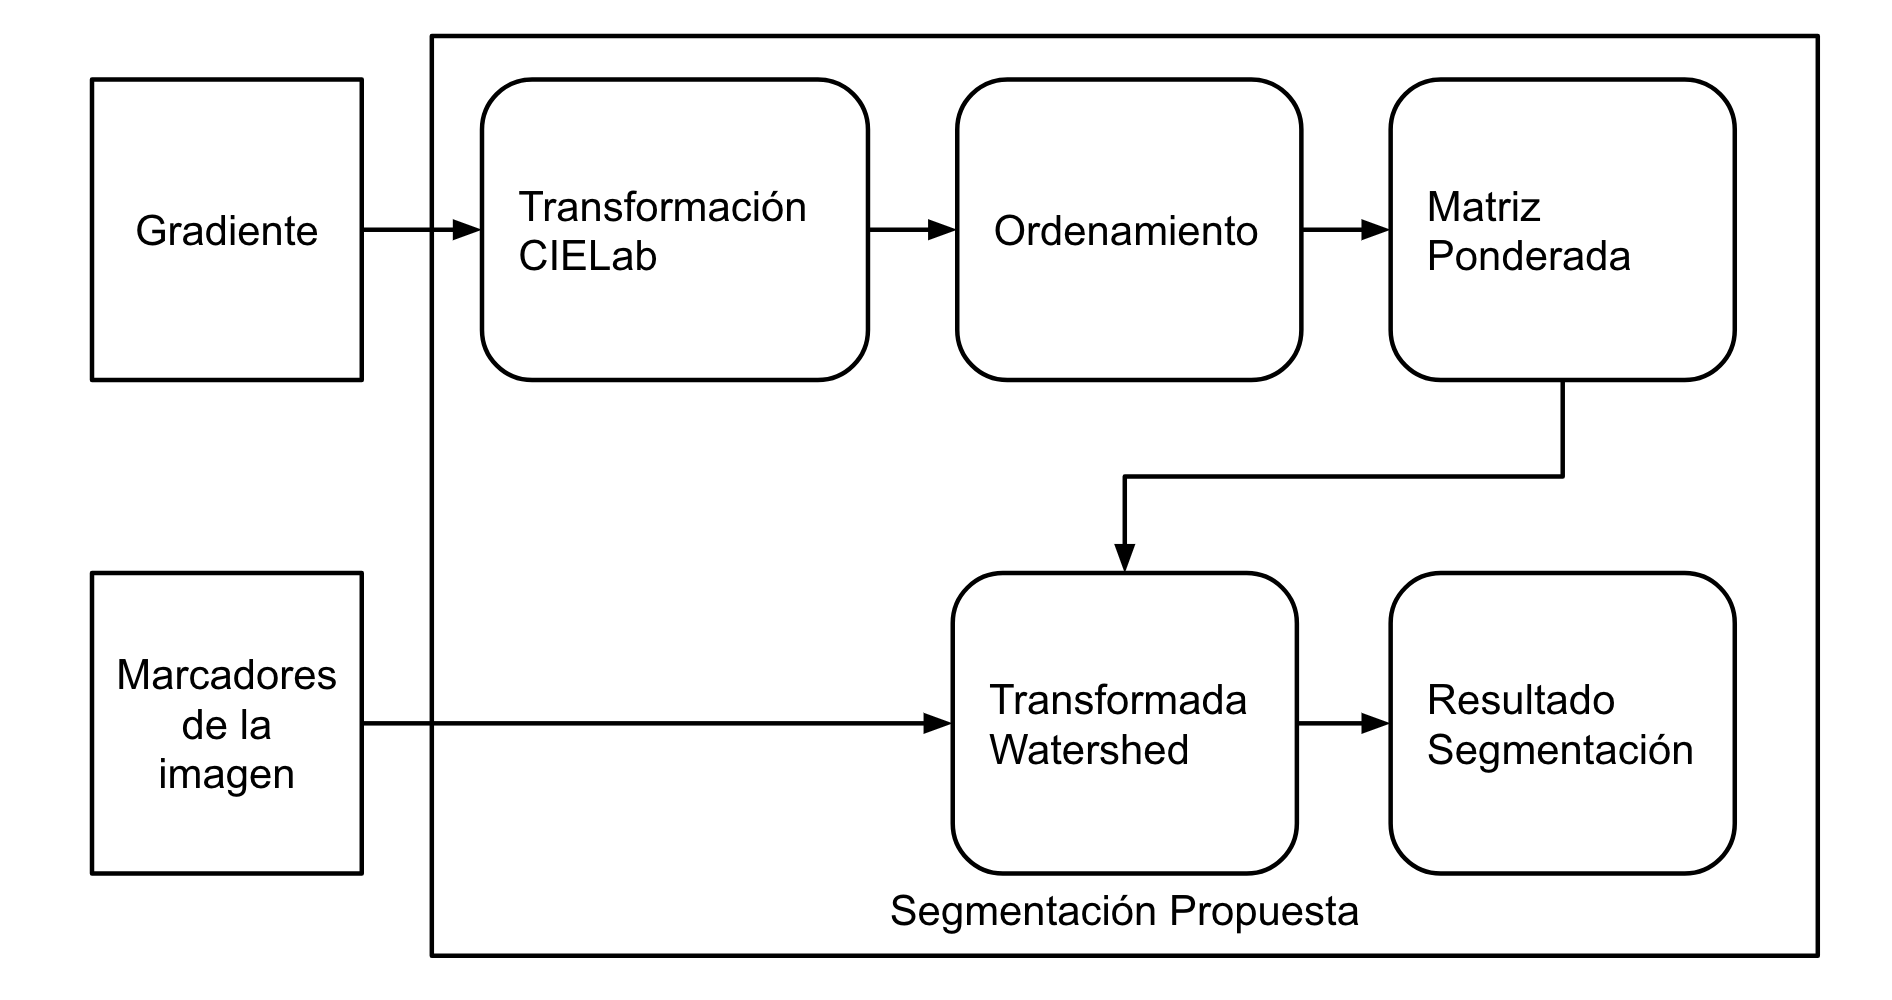
\includegraphics[height=50mm]{./figuras/segmentacion_propuesta.png}
\caption{Flujo de la segmentación propuesta}
\label{img:segpropuesta}
\end{figure*}
\addsymbol{symbol:A}\addsymbol{symbol:B}\addsymbol{symbol:C}
Con el objetivo de ejemplificar el proceso de la segmentación propuesta se utiliza de ejemplo una imagen de tamaño $4 \times 4$. En el Algoritmo \ref{algoritmo} se detallan los pasos a seguir para la realizar la segmentación propuesta de la transformada watershed por inundación con marcadores. Los parámetros de entrada son la gradiente de la imagen y los marcadores como se muestran en la Figura \ref{img:vector-imagen}. A continuación se explica la ejecución del Algoritmo \ref{algoritmo}, donde las variables utilizadas en el texto se encuentran en cursiva para facilitar el seguimiento. 
\begin{figure}[h!]
\centering
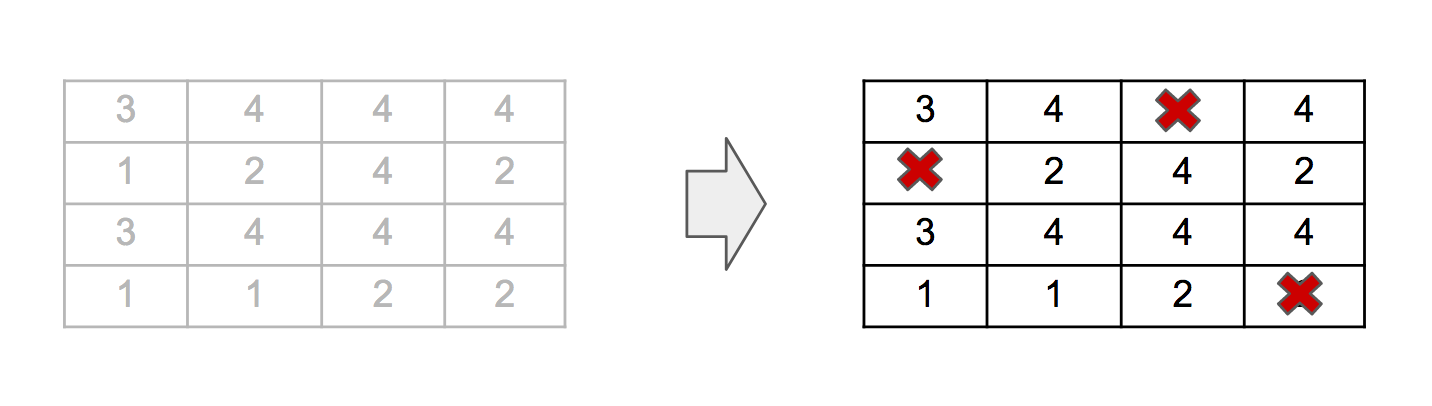
\includegraphics[width=90mm]{./inundacion/inicial.png}
\caption{(a) Gradiente de la imagen, (b) Marcadores de la imagen}
\label{img:vector-imagen}
\end{figure}

Se inicializa una matriz ponderada $transformada$ con los valores por píxel de la transformación de la gradiente del espacio de color RGB a CIELab según la ecuación (\ref{formula:eucli}). En la Figura \ref{img:vector-imagen}(a) se puede ver la representación de la gradiente de una imagen de tamaño $4 \times 4$ en la cual los números representan el valor del píxel luego de asignarle una ponderación basada en el ordenamiento en el espacio de color CIELab.
Los marcadores se colocan en un matriz $marcadores$, con los píxeles (1,3), (2,1) y (4,4). En la Figura \ref{img:vector-imagen}(b) se muestran los marcadores seleccionados de la gradiente de la imagen. 
Para el procesamiento se inicializa una cola de prioridad $lista$ con los marcadores, los cuales son insertados según los valores de la matriz $transformada$ para cada uno de los píxeles en la matriz $marcadores$ como se muestra en la Figura \ref{img:cola-inicio}.
\begin{figure}[h!]
\centering
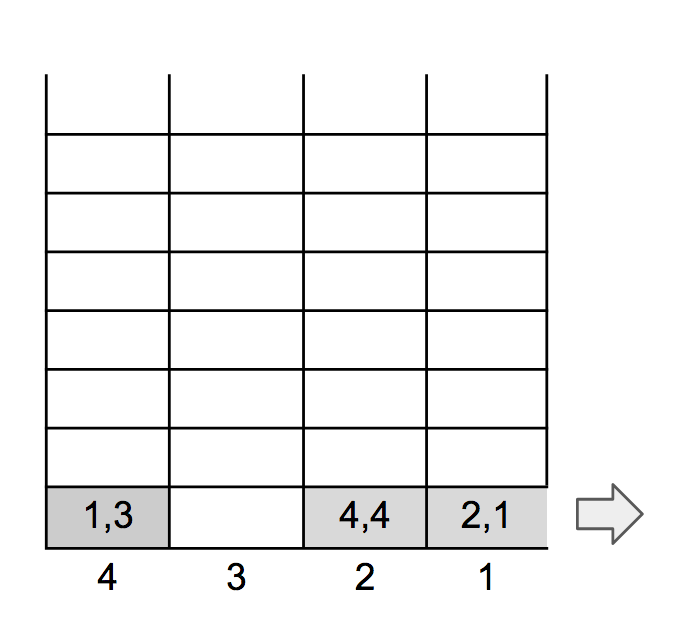
\includegraphics[height=60mm]{./inundacion/cola-inicial.png}
\caption{Inicialización de cola de prioridad}
\label{img:cola-inicio}
\end{figure}
Los píxeles son almacenados en la cola $lista$ de tal forma que el orden (en el cual los píxeles son recuperados de la cola) está dado por dos criterios. El primer criterio esta dado por el nivel en el cual se encuentra el píxel y el segundo está dado por el orden de llegada de los píxeles a su cola. En la Figura \ref{img:prioridad-cola} se muestra una inserción del píxel (2,1) con nivel $1$, teniendo en cuenta los criterios anteriormente citados.
\begin{figure}[h!]
\centering
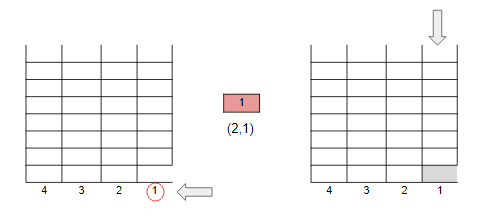
\includegraphics[width=90mm]{./inundacion/prioridad-cola.png}
\caption{(a) Primer criterio de prioridad, (b) Segundo criterio de prioridad}
\label{img:prioridad-cola}
\end{figure}
\SetInd{0.25em}{0.5em}
\renewcommand\bottomfraction{0.85}
\setlength{\textfloatsep}{25pt}
\begin{algorithm2e}
%\setcounter{algocf}{0}% set the counter for the 1st algorithm
\DontPrintSemicolon
%\SetArgSty{textrm}
 \KwIn{Gradiente de la Imagen, Marcadores de la Imagen}
 \KwResult{Imagen Watershed}
  \;
 \Begin{
 Se inicializa una matriz ponderada $transformada$ con los valores por píxel en el espacio de color CIELab según el método de ordenación vectorial reducido con la norma euclidiana.\;
  Se inicializa una matriz $marcadores$ con los marcadores seleccionados.\;
   $lista$ = Cola de prioridad ordenada con los píxeles de $marcadores$ según los valores $transformada[x][y]$.\;
   $pixel$ = $lista.getPixel()$ se obtiene el primer valor de la cola de prioridad.\;
 \Repeat{ $pixel!= NULL$ } {
   $vecinos$ = Se obtienen los vecinos del $pixel$ con conectividad 8.\;
   $posibleEncole$ = Lista para verificar antes de insertar a la $lista$ a procesar.\;
   \ForEach{$vecinos$}{
      \If{$vecino$ no fue procesado} {
      	Se agrega $vecino$ a la lista $posibleEncole$\;
      }
      \If{$vecino$ no está marcado como watershed} {
      	\If{$vecino$ no está marcado} {
      		Se asigna a $pixel$ un nuevo $label$\;
      	}\ElseIf{$vecino$ está marcado con un $label$ distinto a $pixel$}{
      		Se marca el $pixel$ como watershed\;
      	}
      }
   }
   \If{$pixel$ no está marcado como watershed} {
      	Se agrega a $lista$ los píxeles de la lista $posibleEncole$ y se marcan como procesados\;
    }
    \If{$pixel$ no está marcado} {
      	Asignar a $pixel$ el nuevo $label$\;
    }
    $pixel$ = $lista.getPixel()$ se obtiene el siguiente valor de la cola de prioridad.\;
 }
 }
\caption{Segmentación Watershed por Inundación a Color en espacio CIELab}
\label{algoritmo}  
\end{algorithm2e}

El estado inicial de las  etiquetas $A$, $B$ y $C$ para los marcadores mencionados anteriormente, se puede observar en la Figura \ref{img:resultado-inicial} (a). Posteriormente se procesa el primer píxel de la cola de más alta prioridad, en este caso se toma el píxel (2,1), como se puede ver en la Figura \ref{img:cola-inicio}, el cual cuenta con mayor prioridad. 
\begin{figure}[h!]
\centering
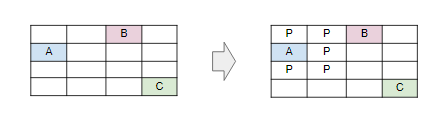
\includegraphics[width=90mm]{./inundacion/resultado-inicial.png}
\caption{(a) Inicialización de etiquetas, (b) Resultado de inundar el píxel (2,1)}
\label{img:resultado-inicial}
\end{figure}
A medida que estos píxeles van siendo procesados, son extraídos de las colas. Dichas colas pueden quedar vacías, lo que implica la eliminación de la misma al momento de la siguiente extracción de píxeles. Por cada $pixel$ extraído, se recorre la lista de $vecinos$ del mismo como se muestran en la Figura \ref{img:cola-vacia} (a), para identificar los que no han sido procesados aún e insertarlos en la cola según el nivel al que corresponde. Los vecinos del píxel en cuestión son analizados antes de incluir a la cola, para ello se utiliza una lista $posibleEncole$ que agrega a la cola todos los vecinos que no hayan sido procesados, pero teniendo en cuenta que el píxel en cuestión no corresponda a las lineas de watershed con la etiqueta $W$. Una vez procesados son marcados con la etiqueta $P$ como se puede observar en la Figura \ref{img:resultado-inicial} (b).
\addsymbol{symbol:P} 
\begin{figure}[h!]
\centering
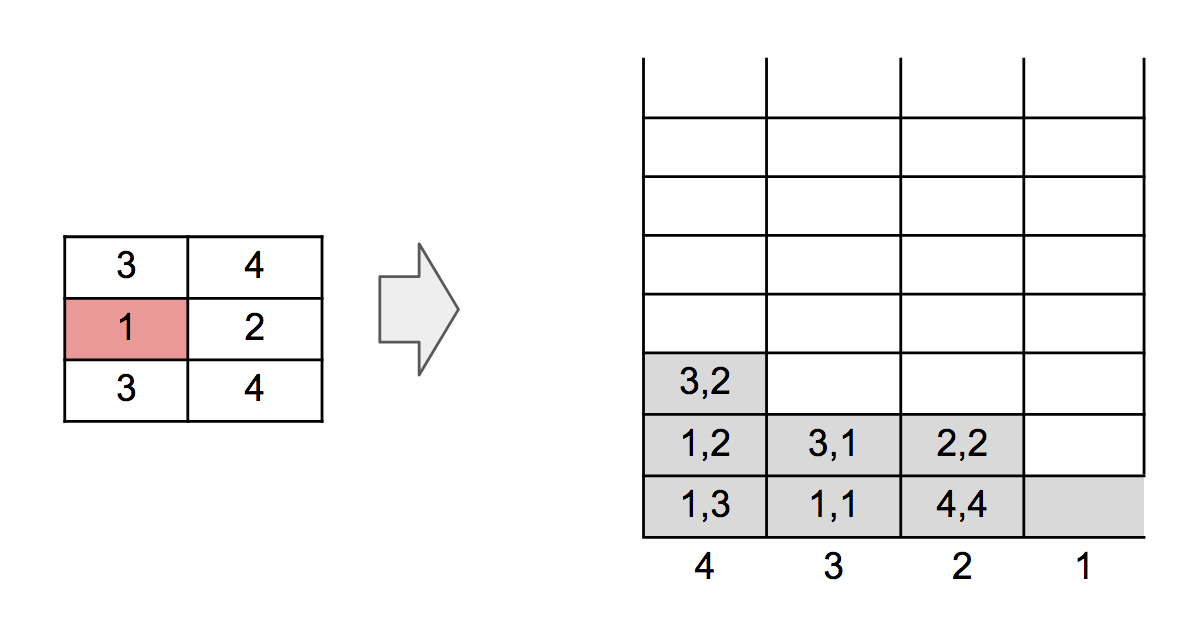
\includegraphics[width=90mm]{./inundacion/cola-vacia.png}
\caption{(a) Vecinos del píxel (2,1), (b) Cola con prioridad mas alta vacía}
\label{img:cola-vacia}
\end{figure}

\begin{figure}[h!]
\centering
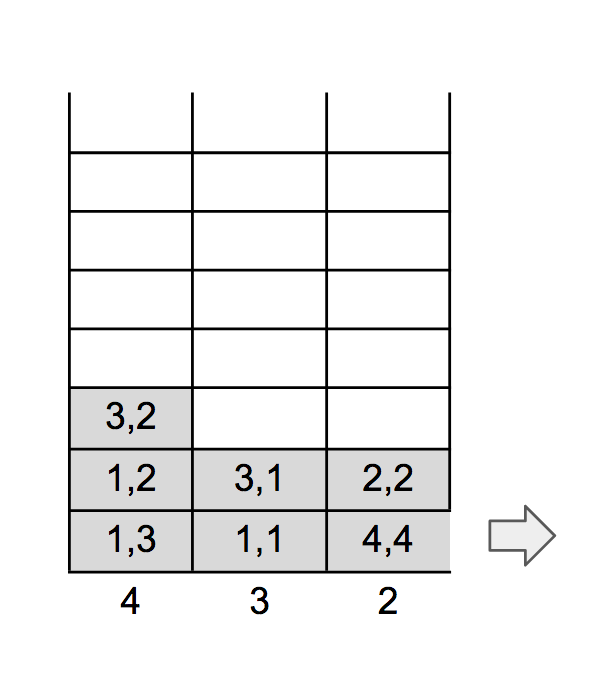
\includegraphics[width=60mm]{./inundacion/cola-eliminada.png}
\caption{Eliminación de cola vacía}
\label{img:cola-eliminada}
\end{figure}

La Figura \ref{img:cola-vacia} (b) muestra el estado de la cola de prioridad luego del procesamiento del píxel (2,1), donde se muestra que la cola de más alta prioridad esta vacía. Cuando un píxel a insertar cuente con una prioridad más alta que la actual, significa que la cola con la prioridad correspondiente ya fue procesada y eliminada, por lo que en dicho caso se debe insertar el píxel en la cola con la prioridad más alta~\cite{Meyer}. En la Figura \ref{img:cola-eliminada} se puede observar que la cola con prioridad 1 ha sido eliminada.
\begin{figure}[h!]
\centering
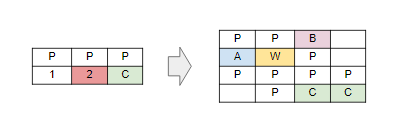
\includegraphics[width=90mm]{./inundacion/unico-label.png}
\caption{(a) Vecinos del píxel (4,4), (b) Etiqueta $C$ asignada en píxel (4,4)}
\label{img:unico-label}
\end{figure}
\begin{figure}[h!]
\centering
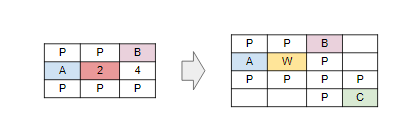
\includegraphics[width=90mm]{./inundacion/varios-label.png}
\caption{(a) Vecinos del píxel (2,2), (b) Etiqueta $W$ asignada en píxel (2,2)}
\label{img:varios-label}
\end{figure}


La etiqueta en una determinada ubicación es determinada de acuerdo a las etiquetas de sus vecinos. En el caso que se cuente solamente con una etiqueta se marca el píxel correspondiente con dicha etiqueta. En la Figura \ref{img:unico-label} (a) se muestran los vecinos del píxel (4,4) y en (b) la asignación de la etiqueta $C$ al píxel (4,4) ya que no existe otra etiqueta diferente. Las vasijas se forman partiendo de los marcadores y se van inundando desde el menor hacia el mayor nivel, según van siendo extraídos de la cola de prioridad. El punto donde se encuentran dos o mas vasijas, es decir, los vecinos cuentan con más de una etiqueta, y no formen parte de la linea de watershed, pasa a formar parte de la linea watershed. En esta ubicación se marca el píxel correspondiente a las lineas de watershed con la etiqueta $W$. 
\addsymbol{symbol:W}
En la Figura \ref{img:varios-label}(a) se muestran los vecinos del píxel (2,2) que poseen etiquetas $A$ y $B$, lo que implica la asignación de la etiqueta W al píxel (2,2) como se muestra en la Figura \ref{img:varios-label}(b).

El proceso se detiene una vez que todos los píxeles de la cola han sido procesados. En la Figura \ref{img:resultado-final} se muestra el estado final de la transformada watershed por inundación.
\begin{figure}[h!]
\centering
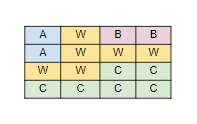
\includegraphics[height=30mm]{./inundacion/resultado-final.png}
\caption{Resultado de la segmentación propuesta}
\label{img:resultado-final}
\end{figure}

A continuación se muestra un ejemplo de la propuesta de este trabajo. Dada una imagen de entrada en RGB como se muestra en la Figura \ref{img:imgprop} se calcula la gradiente marginal, y se seleccionan manualmente los marcadores a ser utilizados para la segmentación.
\begin{figure*}[h!]
\centering
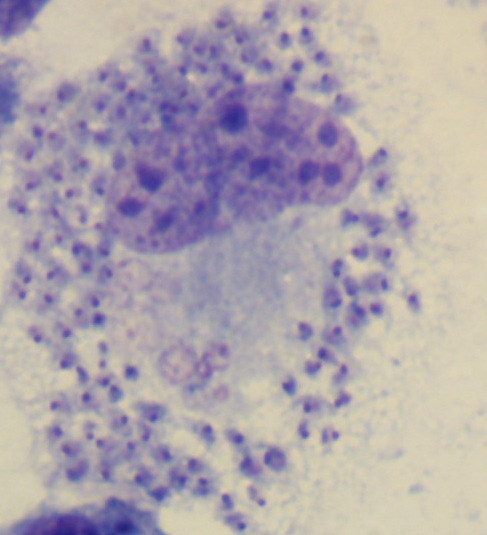
\includegraphics[height=70mm]{./propuesta/cruzi26.jpg}
\caption{Imagen RGB} 
\label{img:imgprop}
\end{figure*}
Los marcadores de la imagen se muestran en La figura \ref{img:imgmark}, donde se marca manualmente cada uno de los objetos deseados.
\begin{figure}[h!]
\centering
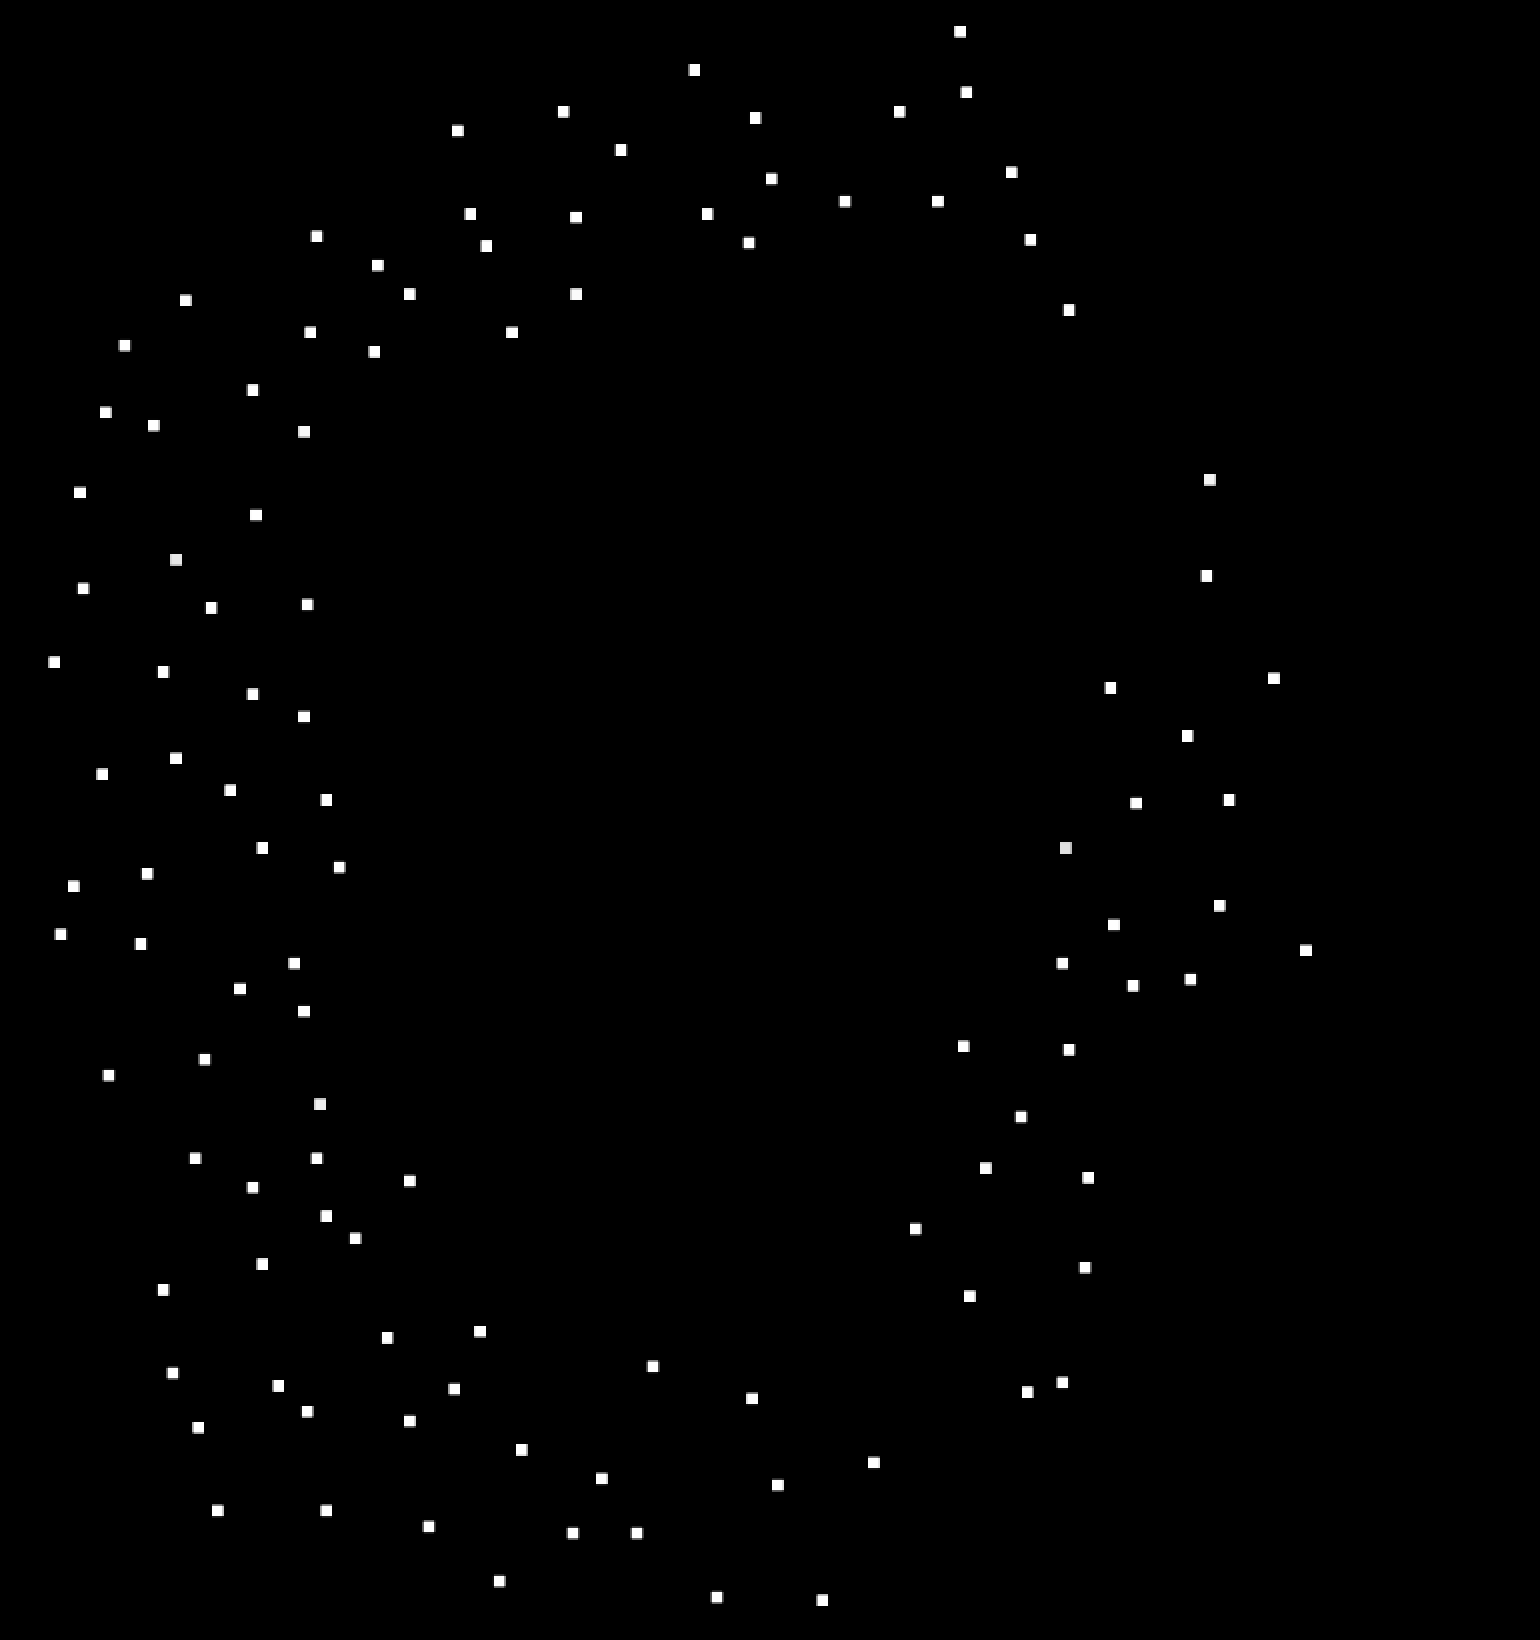
\includegraphics[height=70mm]{./propuesta/marcadores.png}
\caption{Marcadores de la Imagen} 
\label{img:imgmark}
\end{figure}
\begin{figure}[h!]
\centering
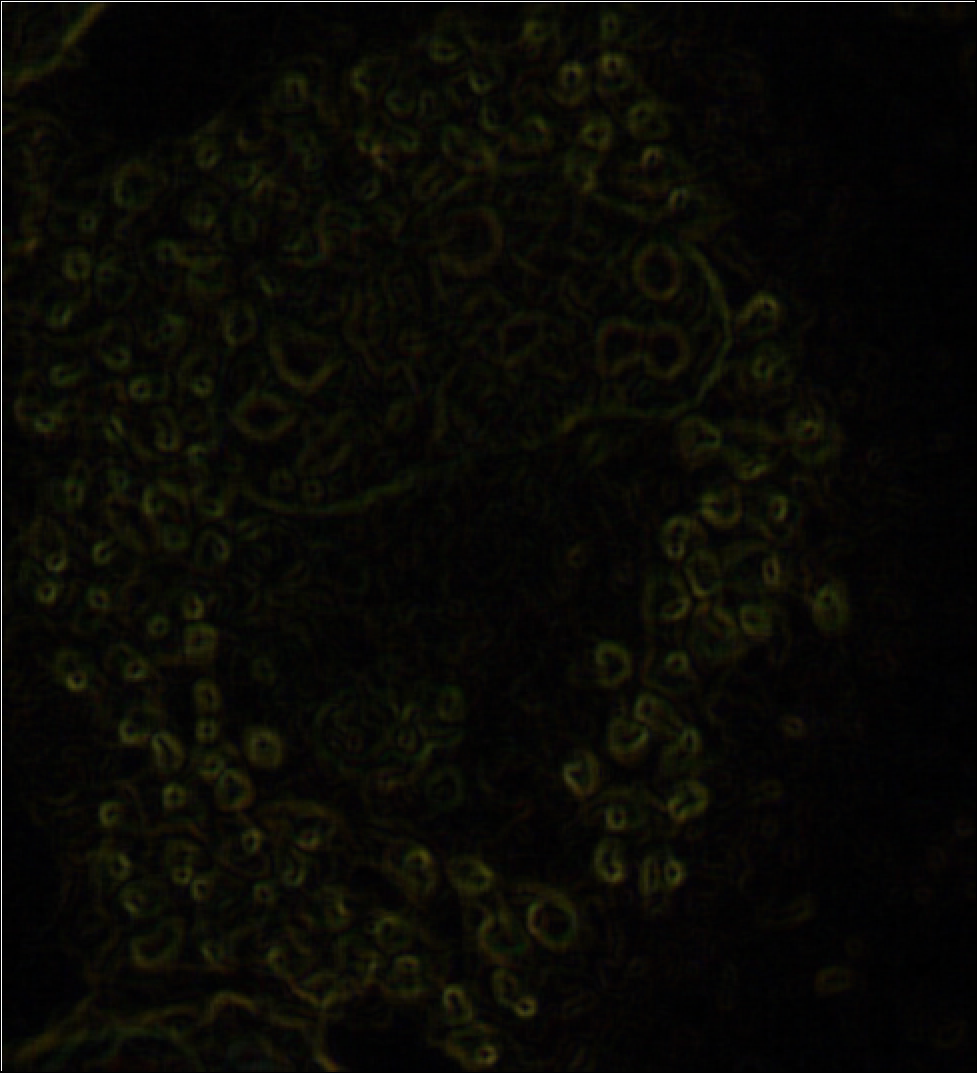
\includegraphics[height=70mm]{./propuesta/gradiente.png}
\caption{Gradiente de la imagen}
\label{img:imggrad}
\end{figure}

La gradiente de la imagen como se muestra en la Figura \ref{img:imggrad} es utilizada para calcular la matriz que será la imagen de entrada para la transformada de watershed. Esta matriz se obtiene calculando para cada píxel un valor escalar que representa el orden en el que se encuentra entre todos los píxeles de la imagen una vez aplicado el ordenamiento  bajo la norma euclidiana según la ecuación (\ref{formula:eucli}). La transformada de watershed utiliza la matriz ponderada y los marcadores pre-seleccionados para realizar la segmentación. 
\begin{figure}[h!]
\centering
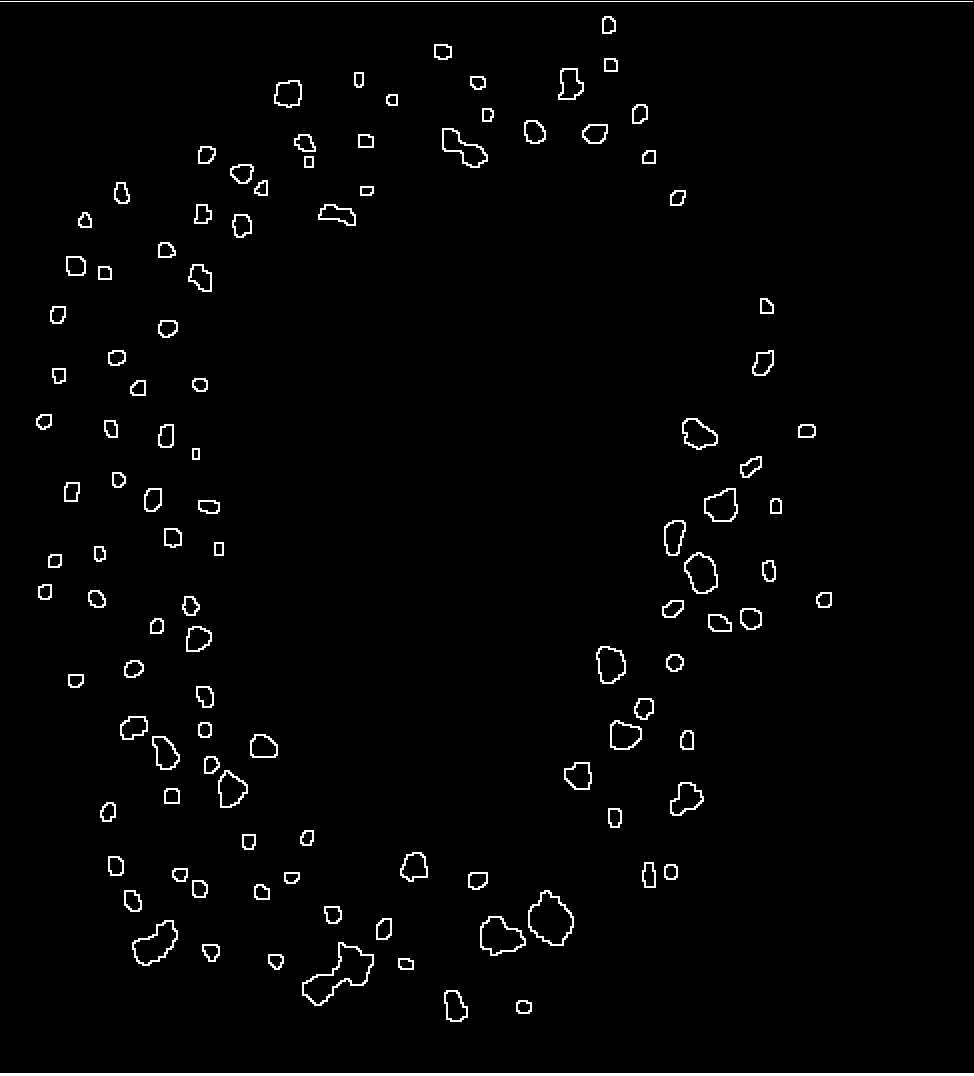
\includegraphics[height=70mm]{./propuesta/relleno.png}
\caption{Resultado de la segmentación de la imagen}
\label{img:imgrelleno}
\end{figure}
\begin{figure*}[h!]
\centering
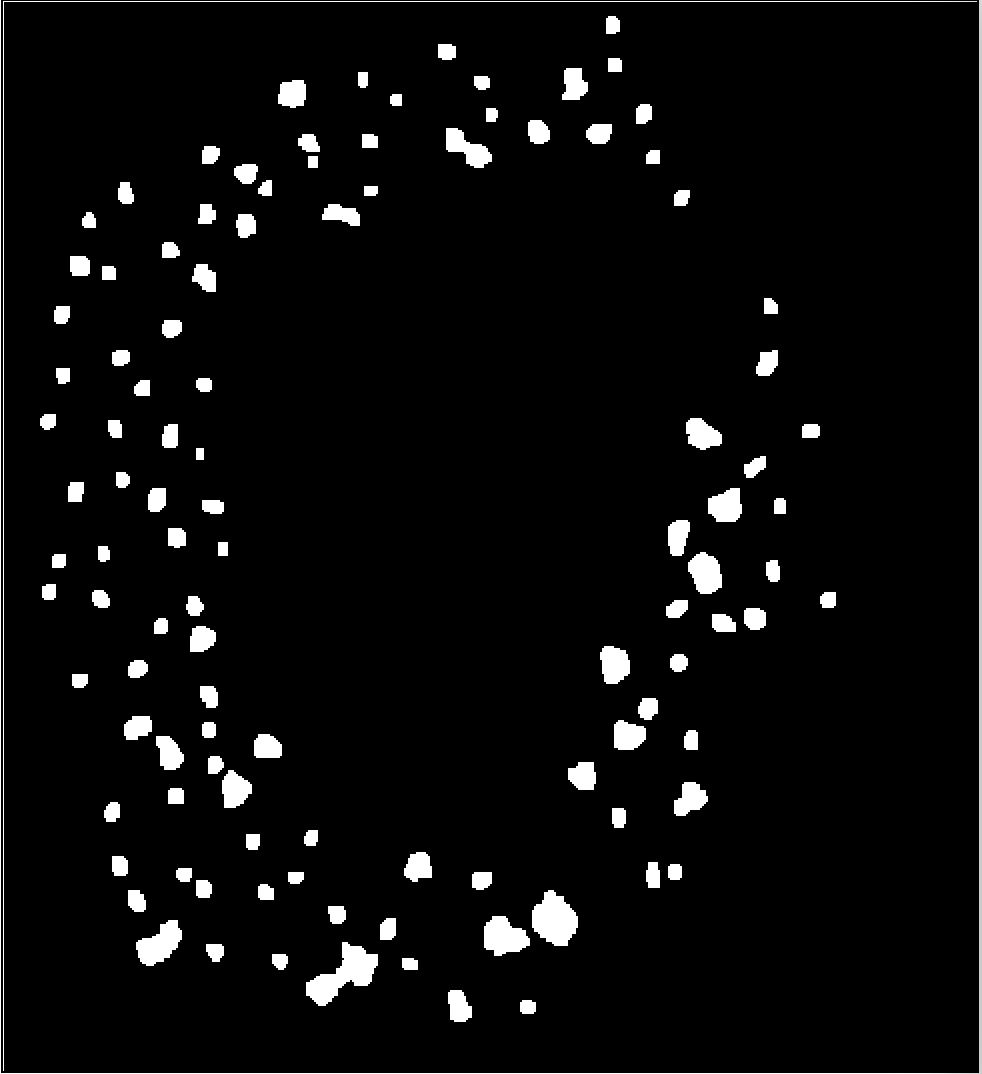
\includegraphics[height=70mm]{./propuesta/resultado.png}
\caption{Resultado de la propuesta de este trabajo}
\label{img:imgresultado}
\end{figure*}
El resultado de la propuesta de este trabajo se muestra en la Figura \ref{img:imgrelleno}, donde están presentes los contornos de los objetos, sobre el cual se aplica un rellenado de agujeros para su mejor visualización, como se puede observar en la Figura \ref{img:imgresultado}. El proceso de relleno de agujeros se encuentra facilitado por el hecho que los resultados contienen objetos cerrados. Este proceso se realiza buscando dichos objetos de izquierda a derecha y posteriormente de arriba a abajo, rellenando así todo su trayecto desde el inicio hasta el final de cada objeto encontrado.
\begin{figure*}[h!]
\centering
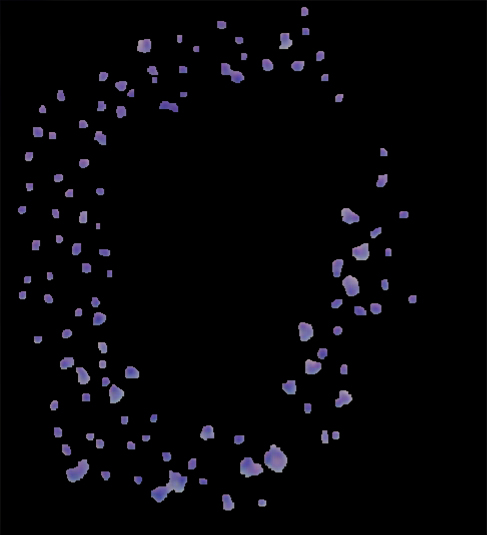
\includegraphics[height=70mm]{./propuesta/amastigotes.jpg}
\caption{Amastigotes segmentados}
\label{img:imgamastigotes}
\end{figure*}

Posteriormente se tiene como resultado final los amastigotes de Trypanosoma cruzi segmentados, como se puede ver en la Figura \ref{img:imgamastigotes}. Los amastigotes segmentados en algunos casos pueden ser más grandes o más pequeños, donde el tamaño ideal de los mismos, el cual es utilizado para la comparación, fue determinado por un especialista. En algunos casos se puede observar que dos o más amastigotes son segmentados como si fuera solo uno. La cuantificación numérica de los resultados para todos los casos obtenidos serán presentados mediante las métricas de evaluación descritas en el próximo capítulo.